%%%%%%%%%%%%%%%%%%%%%%%%%%%%%%%%%%%%%%%%%
% Masters/Doctoral Thesis
% LaTeX Template
% Version 2.5 (27/8/17)
%
% This template was downloaded from:
% http://www.LaTeXTemplates.com
%
% Version 2.x major modifications by:
% Vel (vel@latextemplates.com)
%
% This template is based on a template by:
% Steve Gunn (http://users.ecs.soton.ac.uk/srg/softwaretools/document/templates/)
% Sunil Patel (http://www.sunilpatel.co.uk/thesis-template/)
%
% Template license:
% CC BY-NC-SA 3.0 (http://creativecommons.org/licenses/by-nc-sa/3.0/)
%
%%%%%%%%%%%%%%%%%%%%%%%%%%%%%%%%%%%%%%%%%

%----------------------------------------------------------------------------------------
%   PACKAGES AND OTHER DOCUMENT CONFIGURATIONS
%----------------------------------------------------------------------------------------
\documentclass[
11pt, % The default document font size, options: 10pt, 11pt, 12pt
%oneside, % Two side (alternating margins) for binding by default, uncomment to switch to one side
english, % ngerman for German
singlespacing, % Single line spacing, alternatives: onehalfspacing or doublespacing
%draft, % Uncomment to enable draft mode (no pictures, no links, overfull hboxes indicated)
%nolistspacing, % If the document is onehalfspacing or doublespacing, uncomment this to set spacing in lists to single
%liststotoc, % Uncomment to add the list of figures/tables/etc to the table of contents
%toctotoc, % Uncomment to add the main table of contents to the table of contents
%parskip, % Uncomment to add space between paragraphs
%nohyperref, % Uncomment to not load the hyperref package
headsepline, % Uncomment to get a line under the header
%chapterinoneline, % Uncomment to place the chapter title next to the number on one line
%consistentlayout, % Uncomment to change the layout of the declaration, abstract and acknowledgements pages to match the default layout
]{MastersDoctoralThesis} % The class file specifying the document structure

\usepackage[utf8]{inputenc} % Required for inputting international characters
\usepackage[T1]{fontenc} % Output font encoding for international characters

\usepackage{mathpazo} % Use the Palatino font by default

\usepackage[backend=bibtex,style=authoryear,natbib=true]{biblatex} % Use the bibtex backend with the authoryear citation style (which resembles APA)

\addbibresource{example.bib} % The filename of the bibliography

\usepackage[autostyle=true]{csquotes} % Required to generate language-dependent quotes in the bibliography

%----------------------------------------------------------------------------------------
%   MARGIN SETTINGS
%----------------------------------------------------------------------------------------

\geometry{
    paper=a4paper, % Change to letterpaper for US letter
    inner=2.5cm, % Inner margin
    outer=3.8cm, % Outer margin
    bindingoffset=.5cm, % Binding offset
    top=1.5cm, % Top margin
    bottom=1.5cm, % Bottom margin
    %showframe, % Uncomment to show how the type block is set on the page
}

%----------------------------------------------------------------------------------------
%   THESIS INFORMATION
%----------------------------------------------------------------------------------------

% Your thesis title, this is used in the title and abstract, print it elsewhere with \ttitle
\thesistitle{Aiding Linear Television Media Planning Through Bayesian Inference and Forecasting}
% Your supervisor's name, this is used in the title page, print it elsewhere with \supname
\supervisor{Dr. M.D. \textsc{Voisei}}
% Your examiner's name, this is not currently used anywhere in the template, print it elsewhere with \examname
\examiner{}
% Your degree name, this is used in the title page and abstract, print it elsewhere with \degreename
\degree{Master of Science}
% Your name, this is used in the title page and abstract, print it elsewhere with \authorname
\author{Matthew \textsc{Tiger}}
\addresses{} % Your address, this is not currently used anywhere in the template, print it elsewhere with \addressname

% Your subject area, this is not currently used anywhere in the template, print it elsewhere with \subjectname
\subject{Applied and Industrial Mathematics}
% Keywords for your thesis, this is not currently used anywhere in the template, print it elsewhere with \keywordnames
\keywords{}
\university{\href{https://www.towson.edu/}{Towson University}} % Your university's name and URL, this is used in the title page and abstract, print it elsewhere with \univname
\department{\href{https://www.towson.edu/fcsm/departments/mathematics/}{Department of Mathematics}} % Your department's name and URL, this is used in the title page and abstract, print it elsewhere with \deptname
% Your research group's name and URL, this is used in the title page, print it elsewhere with \groupname
\group{}
% Your faculty's name and URL, this is used in the title page and abstract, print it elsewhere with \facname
\faculty{}

\AtBeginDocument{
\hypersetup{pdftitle=\ttitle} % Set the PDF's title to your title
\hypersetup{pdfauthor=\authorname} % Set the PDF's author to your name
\hypersetup{pdfkeywords=\keywordnames} % Set the PDF's keywords to your keywords
}

\begin{document}

\frontmatter % Use roman page numbering style (i, ii, iii, iv...) for the pre-content pages

\pagestyle{plain} % Default to the plain heading style until the thesis style is called for the body content

%----------------------------------------------------------------------------------------
%   TITLE PAGE
%----------------------------------------------------------------------------------------

\begin{titlepage}
\begin{center}

\vspace*{.06\textheight}
{\scshape\LARGE \univname\par}\vspace{1.5cm} % University name
\textsc{\Large Master's Thesis}\\[0.5cm] % Thesis type

\HRule \\[0.4cm] % Horizontal line
{\huge \bfseries \ttitle\par}\vspace{0.4cm} % Thesis title
\HRule \\[1.5cm] % Horizontal line

\begin{minipage}[t]{0.4\textwidth}
\begin{flushleft} \large
\emph{Author:}\\
{\authorname} % Author name - remove the \href bracket to remove the link
\end{flushleft}
\end{minipage}
\begin{minipage}[t]{0.4\textwidth}
\begin{flushright} \large
\emph{Supervisor:} \\
{\supname} % Supervisor name - remove the \href bracket to remove the link
\end{flushright}
\end{minipage}\\[3cm]

\vfill

\large \textit{A thesis submitted in fulfillment of the requirements\\ for the degree of \degreename}\\[0.3cm] % University requirement text
\textit{at the}\\[0.4cm]
\univname\\[2cm] % Research group name and department name

\vfill

{\large \today}\\[4cm] % Date
%\includegraphics{Logo} % University/department logo - uncomment to place it

\vfill
\end{center}
\end{titlepage}

%----------------------------------------------------------------------------------------
%   DECLARATION PAGE
%----------------------------------------------------------------------------------------

\begin{declaration}
\addchaptertocentry{\authorshipname} % Add the declaration to the table of contents
\noindent I, \authorname, declare that this thesis titled, \enquote{\ttitle} and the work presented in it are my own. I confirm that:

\begin{itemize}
\item This work was done wholly or mainly while in candidature for a research degree at this University.
\item Where any part of this thesis has previously been submitted for a degree or any other qualification at this University or any other institution, this has been clearly stated.
\item Where I have consulted the published work of others, this is always clearly attributed.
\item Where I have quoted from the work of others, the source is always given. With the exception of such quotations, this thesis is entirely my own work.
\item I have acknowledged all main sources of help.
\item Where the thesis is based on work done by myself jointly with others, I have made clear exactly what was done by others and what I have contributed myself.\\
\end{itemize}

\noindent Signed:\\
\rule[0.5em]{25em}{0.5pt} % This prints a line for the signature

\noindent Date:\\
\rule[0.5em]{25em}{0.5pt} % This prints a line to write the date
\end{declaration}

\cleardoublepage

%----------------------------------------------------------------------------------------
%   ABSTRACT PAGE
%----------------------------------------------------------------------------------------

\begin{abstract}
\addchaptertocentry{\abstractname} % Add the abstract to the table of contents
The Thesis Abstract is written here (and usually kept to just this page). The page is kept centered vertically so can expand into the blank space above the title too\ldots
\end{abstract}

%----------------------------------------------------------------------------------------
%   ACKNOWLEDGEMENTS
%----------------------------------------------------------------------------------------

\begin{acknowledgements}
\addchaptertocentry{\acknowledgementname} % Add the acknowledgements to the table of contents
The acknowledgments and the people to thank go here, don't forget to include your project advisor\ldots
\end{acknowledgements}

%----------------------------------------------------------------------------------------
%   LIST OF CONTENTS/FIGURES/TABLES PAGES
%----------------------------------------------------------------------------------------

\tableofcontents % Prints the main table of contents

\listoffigures % Prints the list of figures

\listoftables % Prints the list of tables

%----------------------------------------------------------------------------------------
%   ABBREVIATIONS
%----------------------------------------------------------------------------------------

\begin{abbreviations}{ll} % Include a list of abbreviations (a table of two columns)

\textbf{LAH} & \textbf{L}ist \textbf{A}bbreviations \textbf{H}ere\\
\textbf{WSF} & \textbf{W}hat (it) \textbf{S}tands \textbf{F}or\\

\end{abbreviations}

%----------------------------------------------------------------------------------------

%DEDICATION
%----------------------------------------------------------------------------------------

\dedicatory{For/Dedicated to/To my\ldots}

%----------------------------------------------------------------------------------------
%   THESIS CONTENT - CHAPTERS
%----------------------------------------------------------------------------------------

\mainmatter % Begin numeric (1,2,3...) page numbering

\pagestyle{thesis} % Return the page headers back to the "thesis" style

% Include the chapters of the thesis as separate files from the Chapters folder
% Uncomment the lines as you write the chapters

The authors were tasked by the client with finding the solution to the following
family of differential equations
\[
  \begin{cases}
    -u''(x) + c u(x) = f(x) \\
    0 \leq x \leq 1 \\
    u(0) = \epsilon \\
    u(1) = \delta.
  \end{cases}
\]
Additionally, the client has also requested to be provided with a means of
plotting the solution once obtained.

Throughout this report, the above family of differential equations together with
the interval of definition and initial conditions will be represented by
$Lu = f$ where $L$ can be thought of as the differential operator for the above family.

Assumptions were placed on this family so that $c \in \mathbb{R}$ with $c > 0$
and $f \in C^k([0,1])$ for sufficiently large $k$ so that $f$ is relatively
well-behaved on the defined interval.

In this report we will detail the analytical solution to this family of
differential equations showing that the above problem is well-posed and
explain why this solution is not amenable to practical use. We therefore
provide a numerical scheme to approximate the solution to the family of
differential equations and examine the convergence, consistency and stability
of the numerical scheme. Using the solution provided by the numerical scheme,
we then explore the method for plotting the solution.

In an effort to help researchers glean insight from tweets, Twitter offers
a streaming API that streams all tweets that contain a certain string.
We leverage this service to gather data surrounding the popular television
show \textit{The Walking Dead} and then measure the number of tweets that occur each
hour over a time span.

Using the programming language Python and the library \texttt{tweepy}, a popular
wrapper for the Twitter streaming API, we collected all tweets containing the
hashtag ``\#thewalkingdead'' for three weeks from 2015-11-07 21:00 EST to
2015-11-23 21:00 EST. As this television show airs Sundays at 21:00 EST,
of particular importance is the tweets occurring around this time.
We therefore restrict our measurements to 24 hours prior to and 24 hours after
the television show's airing for the above three week time frame.

These measurements give rise to the time series presented in Figure \ref{tweets_plot}.
From this plot it is clear that, due to the weekly episodic nature of the television
show, there is a seasonal component to this time series. It also appears that
there is a trend component. Thus, in order to fit a stationary time series
to the underlying data, we will need to first apply transformations to the data.

\begin{figure}[!t]
  \centerline{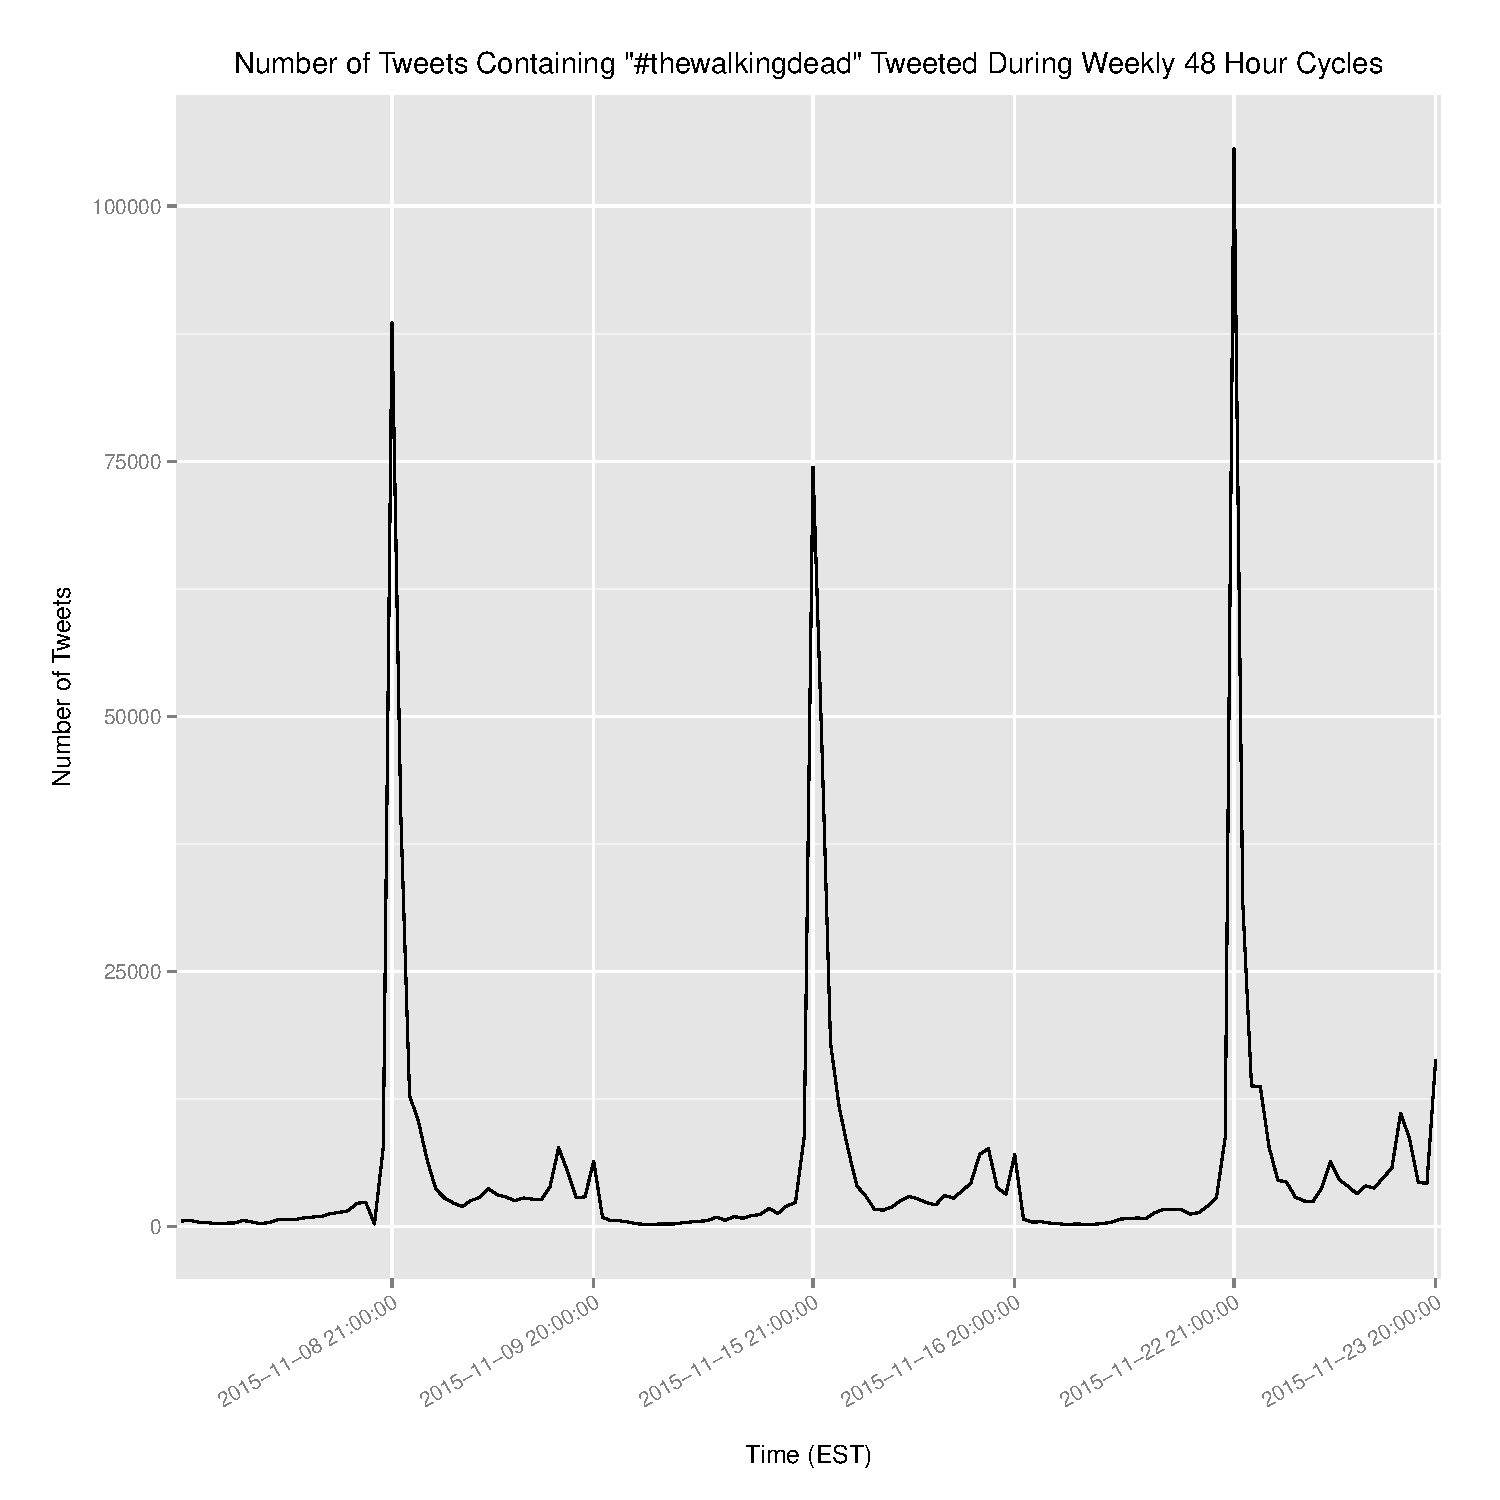
\includegraphics[scale=0.75]{../analysis/plots/tweets_plot}}
  \caption{Time series plot of number of tweets containing the hashtag
  \#thewalkingdead over three 48 hour cycles.}\label{tweets_plot}
\end{figure}

The details behind the process of fitting a stationary time series model to this data is handled in
Section \ref{model}.
%\include{Chapters/Chapter3}
%\include{Chapters/Chapter4}
%\include{Chapters/Chapter5}

%----------------------------------------------------------------------------------------
%   THESIS CONTENT - APPENDICES
%----------------------------------------------------------------------------------------

\appendix % Cue to tell LaTeX that the following "chapters" are Appendices

% Include the appendices of the thesis as separate files from the Appendices folder
% Uncomment the lines as you write the Appendices

%\include{Appendices/AppendixA}
%\include{Appendices/AppendixB}
%\include{Appendices/AppendixC}

%----------------------------------------------------------------------------------------
%   BIBLIOGRAPHY
%----------------------------------------------------------------------------------------

\printbibliography[heading=bibintoc]

%----------------------------------------------------------------------------------------

\end{document}